\chapter{Faraday's Law and Magnetic Induction}
%\section{Magnetic Flux}
%
%%  \textbf{Question:} If a current-carrying wire can generate a magnetic field,
%%  can a magnetic field affect the current in a wire?
%%
%%  \vspace{.3in}\textbf{Answer:} Yes, sort of\ldots
%%
%%  \vspace{.3in}To understand how to \emph{induce} a current by a magnetic field,
%%  we need to look at fluxes again.
%
%
%
%    \pic1{flux2}

Magnetic flux is defined as:
\begin{equation}
  \boxed{\Phi_m=\int_\mathcal{S}\bm B\cdot\dl\bm A}
\end{equation}
where $\bm B$ is the magnetic field, and $\dl\bm A$ is the infinitesimal
area pointing \textbf{outwards}. Note that magnetic flux can also be
expressed as:
\begin{equation}
  \boxed{\Phi_m=\int_{\mathcal S}(\bm B\cdot\hat n)\dl A}
\end{equation}
where $\hat n$ is the outward normal direction
%  

%
%
%
%\begin{frame}{Magnetic Flux Over a Closed Surface}
The SI unit for magnetic flux is a \textbf{weber} (\si\weber), after
German physicist Wilhelm Weber, who invented the electromagnetic telegraph
with Carl Gauss. The unit is defined as:
\begin{equation*}
  \SI1\weber=\SI1{\tesla\metre\squared}
\end{equation*}  
The magnetic flux over any closed surface $\mathcal S$ must always be zero.
This is \textbf{Gauss's law for magnetism}:
\begin{equation}
  \boxed{\oint_{\mathcal S}\bm B\cdot\dl\bm A=0}
\end{equation}
Since magnetic field lines only exist as a loop, that means there should be
equal amount of ``flux'' flowing out of a closed surface as entering the
surface.

Magnetic flux $\Phi_m$ can change due to any of these reasons:
\begin{enumerate}[nosep]
\item A time-dependent magnetic field, i.e. $\bm B=\bm B(t)$
\item A time-dependent surface area, i.e. $\mathcal S=\mathcal S(t)$
\item The orientation of the magnetic field with the surface is
  time-dependentm i.e. $\bm B\cdot\bm A= B\sin\left(\theta(t)\right)\dl A$
\end{enumerate}

\section{Faraday's Law}
\textbf{Faraday's law} states that the time rate of change of magnetic flux
induces electric field $\bm E$ in a circuit, and therefore an
induced electromotive force, or \emph{emf}, $\mathcal E$ (voltage gain):
\begin{equation}
  \boxed{
    \mathcal E=-\oint\bm E\cdot\dl\bm\ell={\color{red}-}
    \diff{\Phi_m}t
  }
\end{equation}
The negative sign {\color{red}highlighted in red} is the result of
\textbf{Lenz's law}, which is related to the conservation energy



\subsection{Example}
A loop of wire is place inside a uniform time-dependent magnetic field
$\bm B_\text{in}(t)$ into the page that is increasing in magnitude in time.
The plane of the loop is perpendicular to $\bm B$.
\begin{figure}[ht]
  \centering
  \begin{tikzpicture}[scale=.35]
    \foreach \xx in {-4.5,-3,...,4.5}{
      \foreach \yy in {-4.5,-3,...,4.5}
      \node at (\xx,\yy) {\color{cyan}$\times$};
    }
    \node[cyan] at (2.75,5.4) {$\bm B_\text{in}$};
    \draw[ultra thick] circle (3);
    
    \draw[ultra thick,fill=magenta!50,opacity=.5] circle (3);
    
    \node[thick,draw=red,fill=red!5,text width=4.8cm]
    (flux) at (-14,2.8){\color{red}
      Magnetic flux through the wire loop into the page is increasing, and
      it is a function of time:
    
      \begin{displaymath}
        \Phi_m(t)=\int_{\mathcal S}\bm B(t)\cdot\dl\bm A=B(t)A
      \end{displaymath}\par
    };
    \draw[thick,->,red] (flux) to[out=0,in=110] (-.75,1.5)
    node[below=-2]{\scriptsize$\mathcal S$};
    
    \node[thick,draw=green!60!black,fill=green!5,text width=4.8cm]
    (emf) at (-14,-4.8){\color{green!60!black}
      An electric field $\bm E$ is generated inside the wire, resulting in
      an induced \emph{emf} $\mathcal E$:
      
      \begin{displaymath}
        \mathcal E=\left|\diff{\Phi_m}t\right|
      \end{displaymath}\par
    };
    %\draw[thick,->,green!60!black] (flux)--(emf);
    \foreach \x in {0,45,90,...,360}
    \draw[rotate=\x,vector,green!60!black] (3,0)--(3,2.5);
    
    \node[thick,draw=blue!70!black,fill=blue!5,text width=4.7cm]
    (curr) at (14,0){\color{blue!70!black}
      An induced current runs in the wire in direction of the electric
      field (Ohm's law):
      
      \begin{displaymath}
        I=\frac{\mathcal E}R
      \end{displaymath}\par
      $R$ is the internal resistance of the wire loop
    };
  %\draw[thick,->,blue!70!black] (emf) to[out=0,in=270] (curr);
  
    \draw[vector,blue!70!black] (2.7,0) arc (0:300:2.7) node[above]{$I$};
  \end{tikzpicture}
\end{figure}

One remaining (and very important) question: how do we know the
direction of the electric field $\bm E$ and current $I$?
%
%
%
\section{Lenz's Law}
To find the direction of the current, we apply \textbf{Lenz's law}:
\begin{center}
  \fcolorbox{black}{yellow!10}{
    \begin{minipage}{.97\textwidth}
      \textbf{LENZ'S LAW:} The induced \emph{emf} and induced current are in
      such are direction as to oppose the change that produces them
    \end{minipage}
  }
\end{center}
The law comes from the conservation of energy, which disallows perpetual
motion machines.
%  %So basically, the conservation of energy

%
%
%
%%\begin{frame}{When Magnetic Flux is Changing}
%%  \begin{itemize}
%%  \item When the magnetic flux $\Phi_m$ is changing, an electromotive force
%%    (\emph{emf}, $\mathcal E$) is created in the wire.
%%  \item Unlike in a circuit, where the \emph{emf} is concentrated at the
%%    terminals of the battery, the induced \emph{emf} is spread across the
%%    entire wire.
%%  \end{itemize}
%%  
%%    \begin{tikzpicture}[scale=.35]
%%      \foreach \xx in {-4.5,-3,...,4.5}{
%%        \foreach \yy in {-4.5,-3,...,4.5}
%%        \node at (\xx,\yy) {\color{cyan}$\times$};
%%      }
%%      \draw[gray,ultra thick] circle (2.9);
%%      \draw[axes,rotate=45] (0,0)--(2.9,0) node[midway,left]{$r$};
%%      \foreach \x in {0,90,...,360} {
%%        \draw[rotate=\x,vector,red] (2.9,0)--(2.9,2.5)
%%        node[pos=0,above left]{$\bm E$};
%%      }
%%    \end{tikzpicture}

%%    \begin{itemize}
%%    \item Since \emph{emf} is work per unit charge, that means that there is an
%%      electric field inside the wire to move the charges.
%%    \item In this example:
%%      \begin{itemize}
%%      \item Magnetic field $\bm B$ into the page
%%      \item The direction of the electric field $\bm E$ corresponds to an
%%        \emph{increase} in magnetic flux
%%      \end{itemize}
%%    \end{itemize}
%%  




\section{AC Generator}

A simple AC (alternating current) generator makes use of the fact that a 
coil rotating against a fixed magnetic field has a changing magnetic flux.
\begin{center}
  \pic{.5}{magnetism2/generator}
\end{center}
Let's say the permanent magnets produce a uniform magnetic field $B$, and the
coil between them has $N$ turns, and an area $A$. Now let's say that the coil
is rotating with an angular frequency $\omega$.

%
%
%
%\begin{frame}{AC Generator}
%  
%    \pic1{generator}

When the coil is turning with an angular frequency $\omega$, the angle
between the coil and the magnetic field is:
\begin{equation*}
  \theta=\omega t+\theta_0
\end{equation*}
The initial angle $\theta_0$ is not important. The magnetic
flux through the coil is given by:
\begin{equation}
  \Phi_m = NAB\cos\theta = NAB\cos(\omega t+\theta_0)
\end{equation}
as the generator turns. The induced \emph{emf} is the rate
of change of magnetic flux:
\begin{equation}
  \mathcal E(t) =\left|\diff{\Phi_m}t\right| =
  \underbracket{NAB\omega}_{\mathcal E_\text{max}}\sin(\omega t+\theta_0)
\end{equation}

%%\begin{frame}{Motional EMF}
%%  
%%    \pic1{motional-emf-1}

%%    When sliding the rod to the right with speed $v$, the magnetic flux through
%%    the loop (and its rate of change) is:
%%
%%      \begin{align*}
%%        \Phi_m &=BA=B\ell x\\
%%        \mathcal E &= \diff{\Phi_m}r = B\ell\diff xt=B\ell v
%%      \end{align*}
%%    
%%    We can use the magnetic force on the charges on the rod to find the
%%    direction of the induced current $I$, and its magnitude is:
%%
%%    \eq{-.15in}{
%%      I=\frac{\mathcal E}R
%%      \end{equation}
%%  
%
%
%
\section{Motional EMF}
What happens when I slide the rod to the right?
\begin{figure}[ht]
  \centering
  \begin{tikzpicture}
    \node {\pic{.45}{magnetism2/motional-emf-1}};

    \fill[magenta!60,opacity=.6] (-2.75,-1.37) rectangle (.97,1.17);
    
    \node[thick,draw=red,fill=pink!30,text width=4cm]
    (phi) at (-4,-3.3){\color{red}
      The magnetic flux through the circuit is given by
      \begin{displaymath}
            \Phi_m=BA=B\ell x
      \end{displaymath}\par
    };
    \draw[axes,red] (phi)--(-1,-.7);
    
    \node[thick,draw=green!60!black,fill=green!10,text width=6.4cm]
    (phi) at (2.5,-3.3){\color{green!60!black}
      When sliding the rod to the right at speed $v$, the rate
      of change in magnetic flux is

      \begin{displaymath}
        \mathcal E = \left|\diff{\Phi_m}t\right| = B\ell\diff xt=B\ell v
      \end{displaymath}\par
    };

    \node[thick,draw=blue!70!black,fill=blue!10,text width=2.5cm]
    (i) at (5,0){\color{blue!70!black}
      This emf induces a current of:
      \begin{displaymath}
        I=\frac{\mathcal E}R
      \end{displaymath}\par
    };
  \end{tikzpicture}
\end{figure}
%%    We can use the magnetic force on the charges on the rod to find the
%%    direction of the induced current $I$, and its magnitude is:
%%
%
%%  

%
%
%
%%\begin{frame}{Motional EMF}
  
\begin{tikzpicture}[scale=1.5,thick]
  \draw (1.5,0) to[battery1,l_=$\mathcal E$] (1.5,1.5)--(0,1.5)
  to[R,l_=$R$] (0,0)--(1.5,0);
\end{tikzpicture}
    
\begin{itemize}
\item An equivalent circuit is shown on the left
\item The amount of current can be found using Ohm's law: $V=IR$
\item Note that the ``motional emf'' produced is spread over the entire
  circuit
  \begin{itemize}
  \item In constrast, in a voltaic cell (or battery), the \emph{emf} is
    concentrated between the two terminals.
  \end{itemize}
\end{itemize}




\section{Lenz's Law}
Something very interesting happens when the current starts running on the
wire.
%\begin{center}
%  \pic{.35}{motional-emf-2}
%\end{center}
It produces an ``induced magnetic field'' out of the page, in the opposite
direction as the field that generated the current in the first place, just
as we expect from Lenz's law.

\begin{figure}[ht]
  \centering
  \begin{tikzpicture}[auto,node distance=105, thick]
    \node[fill=pink!40,font=\large] (a) {
      $\displaystyle\Phi_m=\int_{\mathcal S}\bm B\cdot\dl\bm A$};
    \node[fill=green!20,font=\large] (b) [right of=a] {
      $\displaystyle\left|\diff{\Phi_m}t\right|=\mathcal E$};
    \node[fill=blue!20,font=\large] (c) [right of=b] {
      $I=\dfrac{\mathcal E}R$};
    \node[fill=orange!20,font=\large] (d) [right of=c]{
      $P=I^2R=\dfrac{\mathcal E^2}R$};
    \draw[->] (a)--(b);
    \draw[->] (b)--(c);
    \draw[->] (c)--(d);
    \draw[<-,red] (a)--+(0,-1.3)
    node[draw=red,fill=pink!30,text width=2.7cm,below,font=\scriptsize]{
      Find the loop of circuit and calculate magnetic flux $\Phi_m$ through it
      as a function of time 
    };

    \draw[<-,green!60!black] (b)--+(0,-1.3) node[
      draw=green!60!black,fill=green!10,text width=2.8cm,below,font=\scriptsize
    ]{
      Take time derivative to find the induced \emph{emf} $\mathcal E$
      generated in the circuit loop
    };

    \draw[<-,blue!80!black] (c)--+(0,-1.3) node (cc) [
      draw=blue!80!black,fill=blue!10,text width=2.9cm,below,font=\scriptsize
    ]{
      Apply Ohm's law to find the induced current in the circuit. $R$ can be the
      internal resistance, or a resistor in the circuit
    };

    \draw[<-,orange] (d)--+(0,-1.3) node[
      draw=orange,fill=orange!10,text width=3.2cm,below,font=\scriptsize
    ]{
      Calculate power dissipated in the circuit, and compare to the
      power input
    };

    \node[fill=gray!20,draw=black,font=\scriptsize,text width=7.2cm]
    (I) at (1.9,-3.9) {Direction of induced current $I$ must produce a magnetic
      field that opposes the change in magnetic flux.
      \begin{itemize}
      \item If $\Phi_m$ is increasing, magnetic field must decrease it
      \item If $\Phi_m$ is decreasing, magnetic field must increase it
      \end{itemize}\par
    };
    \draw[->] (cc) to[out=270,in=0] (I);
  \end{tikzpicture}
\end{figure}



\section{Inductance}

\subsection{Back \emph{emf}}
Consider a very simple circuit consisting of a voltage source and a coil
\begin{center}
  \begin{tikzpicture}[american voltages,scale=1.3,thick]
    \draw (0,0) to[battery1,l=$\mathcal E$] (0,1.5)
    to[short,-*] (.5,1.5);
    \draw (.55,1.7) to[short,*-*] (1,1.5)--(1.5,1.5) to[L] (1.5,0)--(0,0);
  \end{tikzpicture}
\end{center}
\begin{itemize}
\item When the switch is closed and current begins to flow, the coil
  begins to generate a magnetic flux inside
\item As the current changes (initially increasing with time), it
  self-induces a ``back \emph{emf}'' that opposes the change in current
\item A current can't jump from zero to some value (or from some value to
  zero) instantaneously
\end{itemize}

%
%
%
%\begin{frame}{Back \emph{emf}}
\begin{center}
  \begin{tikzpicture}[american voltages,scale=1.3,thick]
    \draw (0,0) to[battery1,l=$\mathcal E$] (0,1.5)
    to[short,-*] (.5,1.5);
    \draw (.55,1.7) to[short,*-*] (1,1.5)--(1.5,1.5) to[L] (1.5,0)--(0,0);
  \end{tikzpicture}
\end{center}
\begin{itemize}
\item Breaking the circuit causes the magnetic flux to change very rapidly
\item The rapid change of $\Phi_m$ creates a large induced back \emph{emf}
  that is proportional to the time rate of change of magnetic flux
  $\Phi_m'(t)$
\item The back \emph{emf} creates a large voltage drop across the switch
\item Large voltage across two metal contact produces a very strong electric
  field--strong enough to tear electrons away from air molecules
  (``dielectric breakdown'')
\item Air conducts electricity in the form of a ``spark''
\end{itemize}

%
%
%
%\begin{frame}{Self Inductance}
A solenoid carrying a current generates a magnetic field $B$; its magnitude at
the core is proportional to the current $I$:
\begin{equation}
  B=\left[\frac{\mu_0N}\ell\right]I
\end{equation}
Since $\bm B\propto I$, the magnetic flux through the core of the solenoid
(really $\Phi_m=NBA$, where $A$ is the cross-sectional area of the solenoid
and $N$ is the number of coils) is therefore also proportional to $I$, i.e.
\begin{equation}
  \boxed{\Phi_m=LI}
\end{equation}
where $L$ is the called the \textbf{self inductance} of the coil.

%
%
%
%\begin{frame}{Self Inductance}
For a solenoid, we can see that the self inductance is given by:
\begin{equation}
  \boxed{L=\frac{\Phi_m}I=\mu_0 n^2A\ell}
\end{equation}

\begin{center}
  \begin{tabular}{l|c|c}
    \rowcolor{pink}
    \textbf{Quantity} & \textbf{Symbol} & \textbf{SI Unit} \\ \hline
    Self inductance & $L$ & \si\henry\\
    Vacuum permeability & $\mu_0$ & \si{\tesla.\metre\per\ampere} \\
    Number of coils per unit length & $n$ & \si\ampere \\
    Cross-section area of the solenoid & $A$ & \si{\metre\squared} \\
    Length of the solenoid & $\ell$ & \si\metre
  \end{tabular}
\end{center}
Note that $A\ell$ is the \emph{enclosed volume} of the solenoid. The SI unit
for self inductance is a \textbf{henry} (\si\henry).

%
%
%
%\begin{frame}{Self Inductance and Induced EMF}
If the current changes, the magnetic flux changes as well, therefore inducing
an electromotive force in the circuit According Faraday's law:
\begin{equation}
  \boxed{
    \mathcal E=-\diff {\Phi_m}t=-L\diff It
  }
\end{equation}
The self-induced \emph{emf} is proportional to the rate of change of current

%
%
%
\subsection{Magnetic Energy}
At any instant, the magnitude of the induced emf is
\begin{equation}
  \mathcal E=L\diff It
\end{equation}
so the power absorbed by the inductor is
\begin{equation}
  P(t)=\mathcal EI=LI\diff It
\end{equation}
Integrating in time gives the magnetic (potential) energy that is stored in
the magnetic field:
\begin{equation}
  U_m
  =\int_0^t P(t)\dl t
  =L \int I\diff It \dl t
  =L \int_0^I I\dl I=\frac12LI^2
\end{equation}



%\begin{frame}{Magnetic Energy}
Just as a capacitor stores energy in its electric field, an inductor coil
carrying a current $I$ stores energy in its magnetic field, given by:
\begin{equation}
  \boxed{U_m=\frac12LI^2}
\end{equation}
We can also define a \textbf{magnetic energy density}:
\begin{equation}
  \boxed{\eta_m=\frac{B^2}{2\mu_0}}
\end{equation}

